\chapter{Quick start} \label{cha:quickstart}

This chapter guides you step by step towards the complete configuration of a project using a predefined
configuration provided with the package (setup for \NO2 retrieval from ground-based \glslink{maxdoas}{MAXDOAS} measurements).
The retrieval settings are those recommended during the \glslink{cindi}{CINDI} intercomparison campaign (see \citet{Roscoe2010}).

\section{Creating a project to browse spectra}

\subsection{Creating a New Project}

When QDOAS starts on an empty application, the user interface looks like~:

\hfill\vspace{-.8\baselineskip}
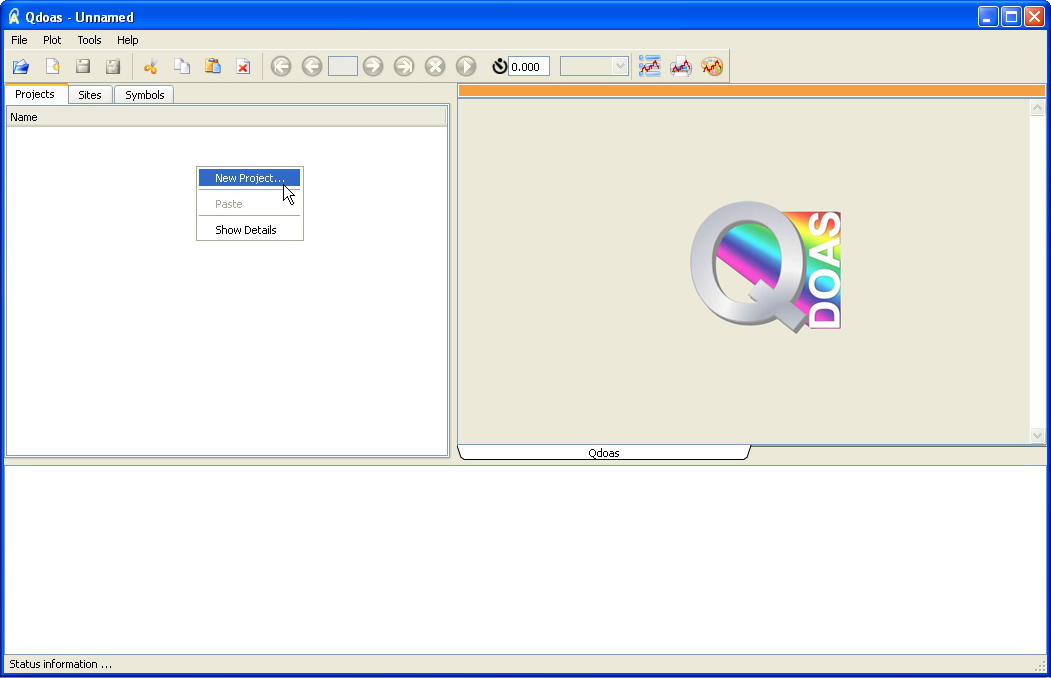
\includegraphics[width=\textwidth]{img/Quickstart_New.jpg}

From the upper-left panel, right-click the \textbf{New Project} option, and give it a name, for example MAXDOAS-VIS
as the purpose of the application here is to retrieve \NO2 from MAXDOAS measurements in the visible region.

\begin{minipage}{\textwidth}
\subsection{Project properties}
\hfill\vspace{-.8\baselineskip}
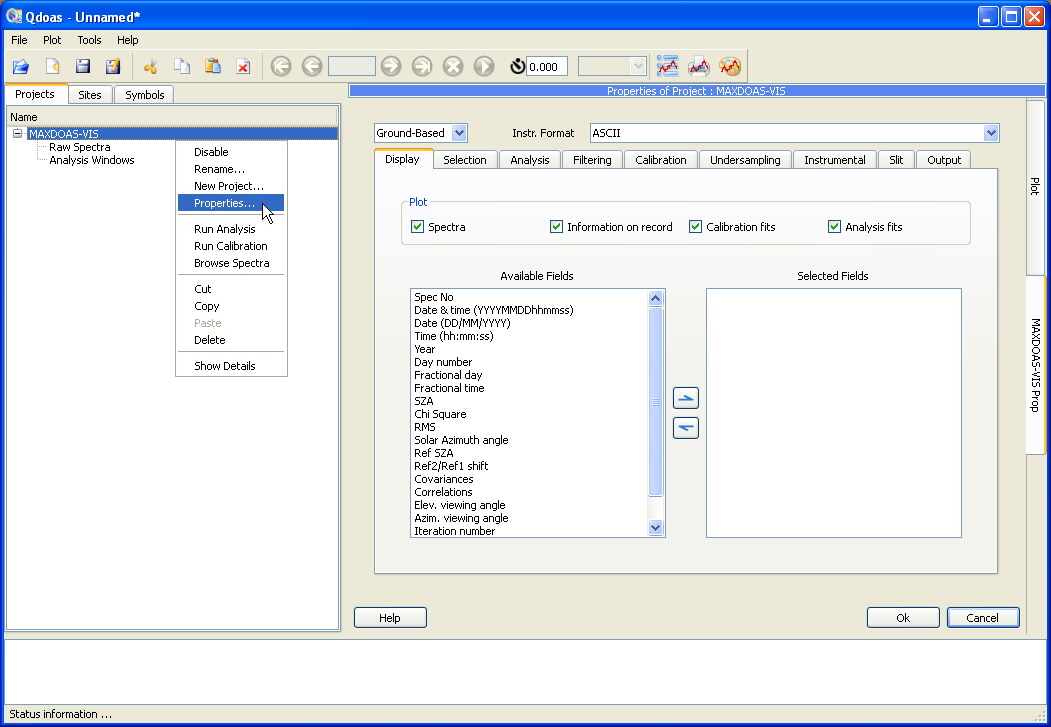
\includegraphics[width=\textwidth]{img/Quickstart_ProjectProperties.jpg}
\end{minipage}\\

From the MAXDOAS-VIS tree node, right-click \textbf{Properties} to open the \textbf{Properties} dialog box on the upper-right panel.
Switch to the \textbf{``Instrumental"} page to complete information on the format of the files to read.  The default file format
(\textbf{Ground-based, ASCII}) is correct for the example~:

\hfill\vspace{-.8\baselineskip}
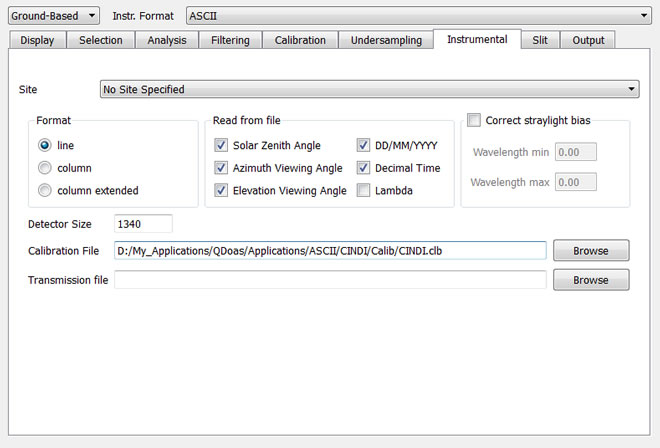
\includegraphics[width=\textwidth]{img/Quickstart_ProjectInstrumental.jpg}

The detector size has to be specified.  The files in the example contain one  record per line and the following information are given in the expected order~:

\begin{minipage}[t]{\textwidth}
\vspace{-1\baselineskip}
\begin{itemize} \itemsep -6pt
\item Solar Zenith Angle
\item Azimuth Viewing Angle
\item Elevation Viewing Angle
\item Date in the DD/MM/YYYY (day/month/year) format
\item Fractional time
\end{itemize}
\end{minipage}
\vskip 6pt

The wavelength calibration is provided in a separate file.

Switch back to the \textbf{``Display"} page to select information you want to see when browsing spectra and click ok to save \textbf{Projects properties}~:

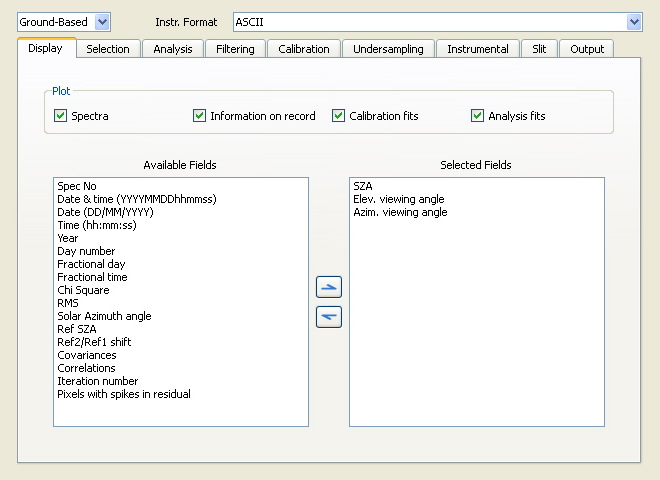
\includegraphics[width=\textwidth]{img/Quickstart_ProjectDisplay.jpg}

\subsection{Inserting Files}

To insert files under the new project, right-click \textbf{Insert File} or \textbf{Insert Directory} from the \textbf{Raw Spectra} node.
We prefer to select the directory~:

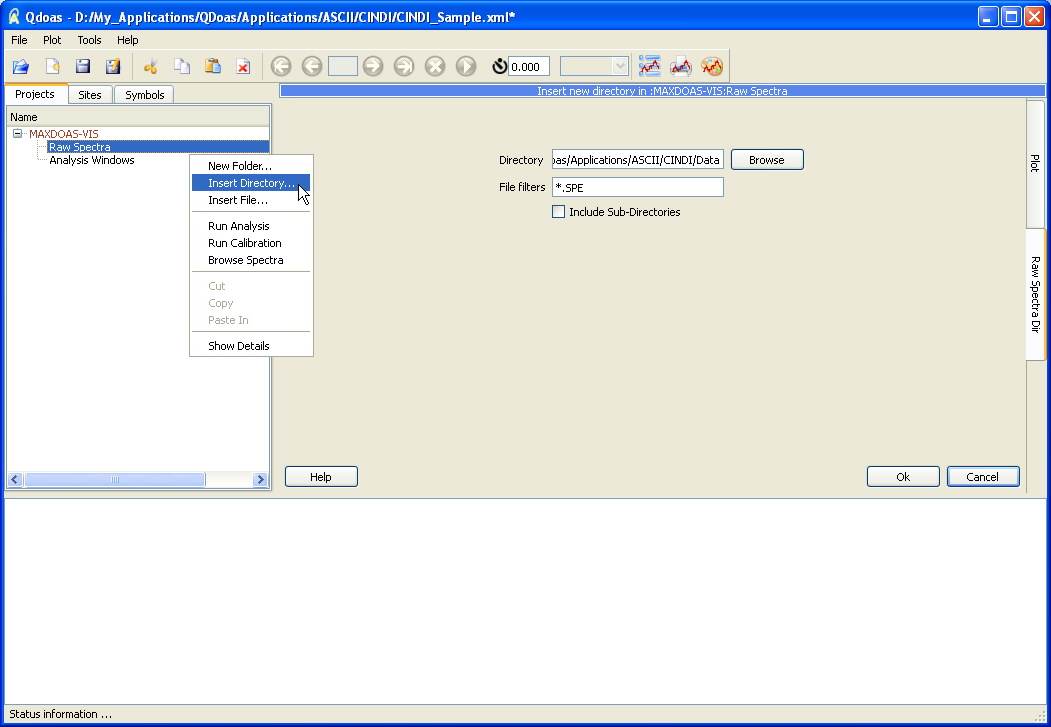
\includegraphics[width=\textwidth]{img/Quickstart_InsertFiles.jpg}

\subsection{Browsing Files}

Right-click the \textbf{Browse Spectra} option from the \textbf{Data directory} name to browse spectra ~:

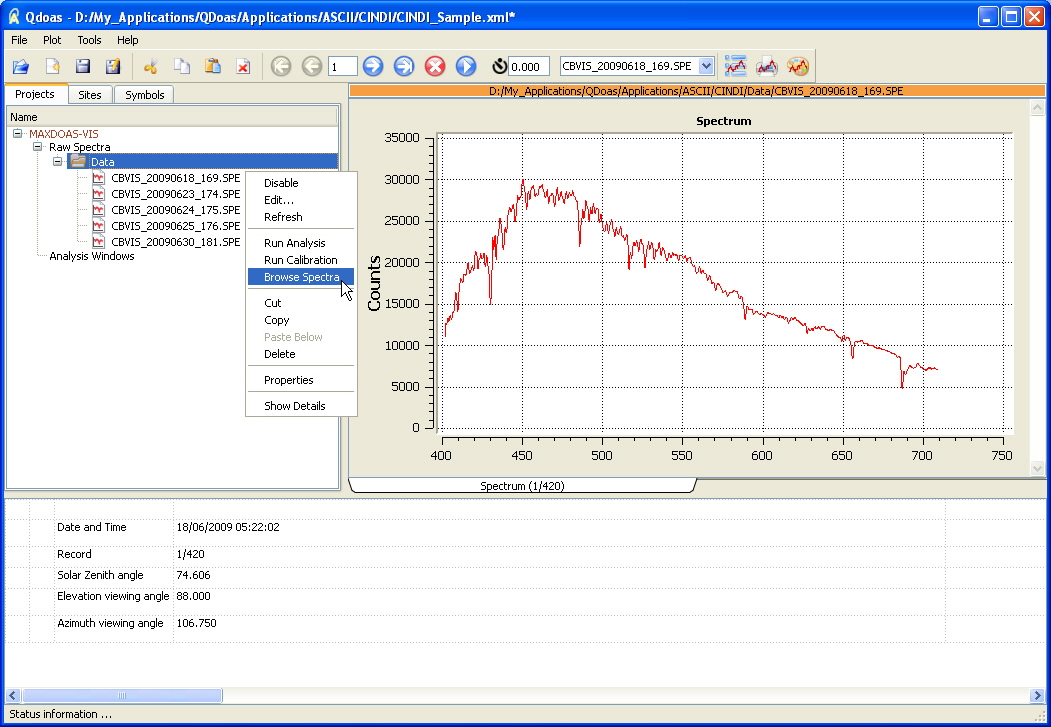
\includegraphics[width=\textwidth]{img/Quickstart_BrowseSpectra.jpg}

Buttons of the toolbar allow moving from one record to the other but also to switch to another file of the directory (possible if the
\textbf{Browse spectra} option has been clicked from the root directory and not from a file).


\subsection{Handling Graphs}

Zoom is possible by right-clicking the \textbf{Interactive} option from the \underline{\textbf{plot title}}~:

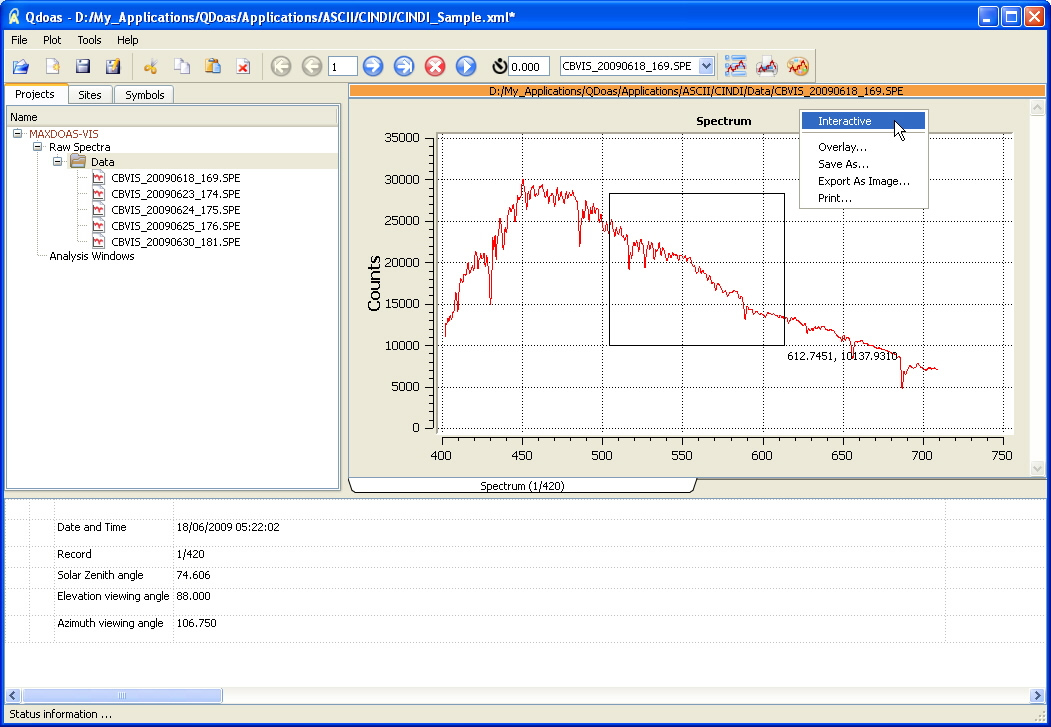
\includegraphics[width=\textwidth]{img/Quickstart_PlotZoom.jpg}

Other options such as export the plot in ASCII (\textbf{Save As}) or PNG (\textbf{Save As Image}) are also available.  Reference spectra used in the retrieval can be saved in ASCII by this way.

\subsection{Saving Your Work}

Be sure to save your work regularly using \textbf{File $\rightarrow$ Save} or  \textbf{File $\rightarrow$ SaveAs}.
The format of configuration files is XML.  Always use the \textbf{Stop} button (cross in a red circle) in the toolbar before coming back
to the project configuration.

\section{Example~: Configuration of a project for \NO2 retrieval}

\subsection{Configuring A Project For Spectra Analysis}

The configuration of a project requires the following steps~:

\begin{qdoasitem}
\item define all symbols related to the cross sections files that will be used in the analysis;
\item call back the \textbf{Projects properties} dialog box to parameterise the wavelength calibration procedure and to setup analysis options independent of the spectral window (fitting method, unit for shifts);
\item create an \textbf{`Analysis Window'} item in the \textbf{Projects} tree for each spectral window to process, and parameterise it.
\end{qdoasitem}

These steps are described through the example file \textbf{CINDI\_Sample.xml} provided with the package.

\subsection{Description of CINDI\_Sample.xml}

The file \textbf{CINDI\_Sample.xml} contains the configuration of a project for \NO2 retrieval.
Before using the file, you may change the paths according to your installation.  The fastest way to do it is to
edit the file and replace all \textbf{D:/My\_Applications/QDoas/Applications/ASCII/CINDI} according to your installation.
Then, use \textbf{Files $\rightarrow$ Open} command from the QDOAS menu bar or the equivalent button in the toolbar to load the application.

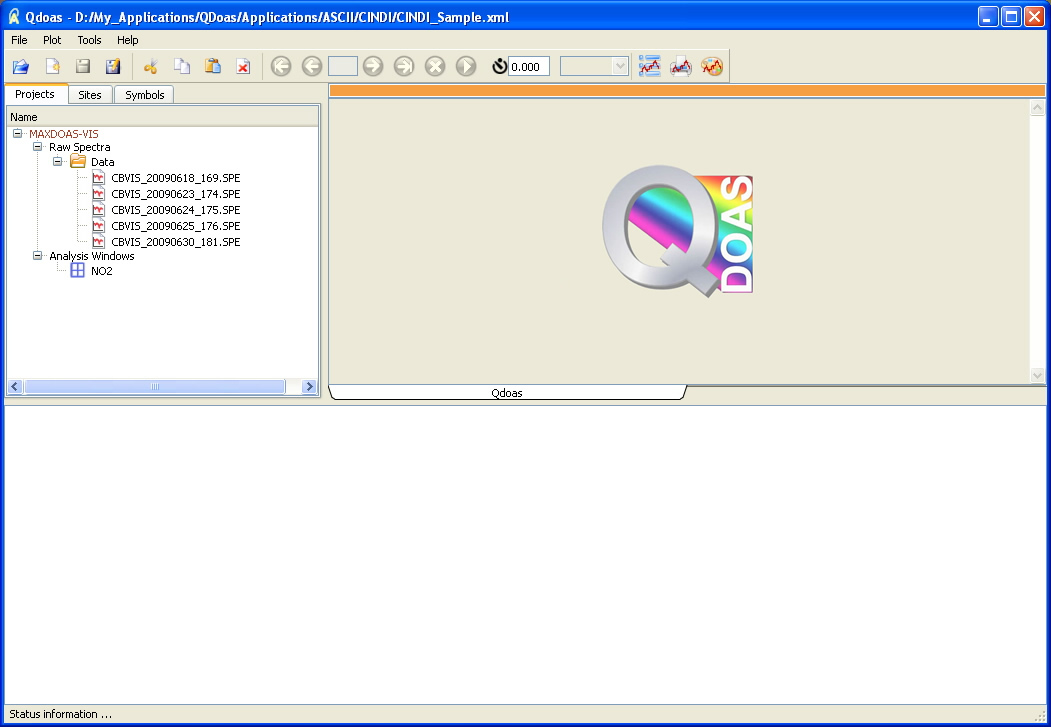
\includegraphics[width=\textwidth]{img/Quickstart_Project.jpg}

\subsection{Settings For NO$_{2}$ Retrieval} \label{sec:no2_settings}

\textbf{Calibration interval}~: depends on the wavelength range covered by the detector.  It should include all spectral windows.
In our application, we have selected 405-580 nm.  A preliminary calibration has been previously measured in laboratory and already
improved with the wavelength calibration procedure of QDOAS (see section \ref{sec:wavel-calibr})

\textbf{Spectral window}~: 425-490 nm;

\textbf{Main Cross sections}~:

%\hfill\vspace{.8\baselineskip}
\begin{longtable}{ l p{6cm} l }
     & \textbf{Source} & \textbf{Files} \\
   \textbf{O$_3$} & \citet{Bogumil2003}, 223 K	& o3\_223K\_Bogumil.xs \\
	  \textbf{NO$_2$}	& \citet{vandaele1996}, 298 K et 220 K	& no2\_298K\_vanDaele.xs \\
   & & no2a\_220K\_vanDaele.xs \\
	  \textbf{O$_4$} & Hermans et al.	& o4\_Hermans\_web.xs\\
	  \textbf{H$_2$O} & From HITRAN data base	& h2o\_hitran.xs \\
	  \textbf{Ring} &	Ratio of the rotational raman spectrum by the solar one,  both convolved at the resolution of the instrument with the \textbf{Convolve Ring} option.	& Ring\_NDSC2003.xs
\end{longtable}

The cross sections are those recommended during the \glslink{cindi}{CINDI} intercomparison campaign (see \citet{Roscoe2010}).

\subsection{Defining Symbols}

The first thing to do is to define the cross sections symbols according to the files names (see table above)~: O3, NO2, NO2a, O4, H2O, Ring
(the case is not important).  A description can be added.  QDOAS needs these symbols for internal use.

\begin{center}
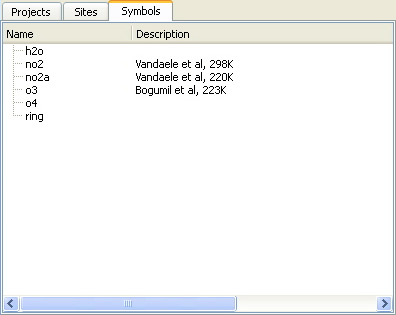
\includegraphics[scale=0.5]{img/Quickstart_Symbol.jpg}
\end{center}

\begin{minipage}{\textwidth}
\subsection{Projects Properties}\hfill
\vspace{-0.8\baselineskip}
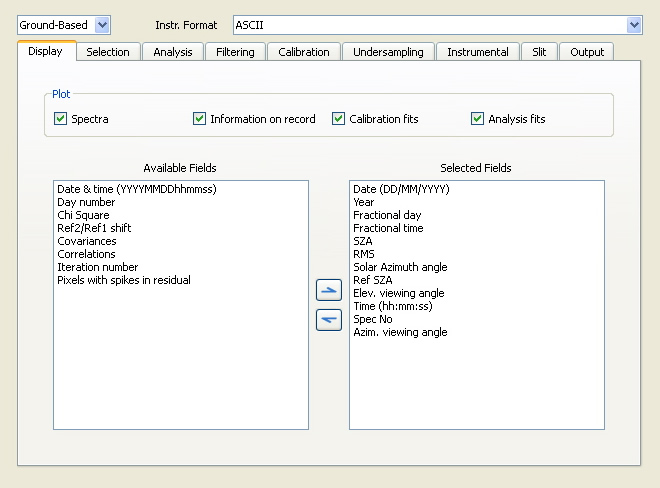
\includegraphics[width=\textwidth]{img/Quickstart_DisplayPage.jpg}
\end{minipage}

Go back to the \textbf{Projects tree} and right-click the \textbf{Properties} command from the MAXDOAS-VIS
node to open the \textbf{Projects properties} dialog box.  The \textbf{Display} tab page appears first.
Some additional fields related to the analysis can be selected such as the  \glslink{rms}{\textbf{RMS}} or the reference spectrum \gls{sza} (\textbf{Ref SZA})~:

\subsubsection{Calibration Parameterisation}\label{sec:calibr-param}
In the example, the \textbf{Calibration} page is configured as follows~:

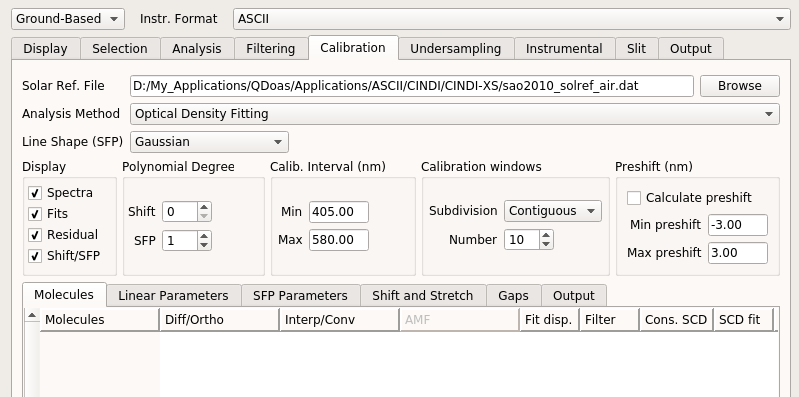
\includegraphics[width=\textwidth]{img/Project_Calibration.png}

\begin{description}
\item[Solar ref. file] Use this button to locate the solar spectrum
  (in this case, a high-resolution one because the slit function is
  fitted, otherwise a solar spectrum previously convolved at the
  resolution of the instrument).
\item[Analysis Method] The fitting method used for wavelength
  calibration can be different from the one selected for spectra
  evaluation in the \textbf{Analysis tab page}.
\item[Line Shape (SFP)] This button is checked in order to fit the
  resolution of the slit function; in this case, a Gaussian line shape
  is selected.
\item[Display] Check boxes in the frame to display the indicated
  graphs.
\item[Polynomial degree] The degree of the polynomial used in the
  final determination of the wavelength registration (shift) and the
  wavelength-dependent slit function (SFP).
\item[Calib.\ Interval (nm)] The complete calibration interval.
\item[Calibration windows] The number of calibration subwindows, as
  well as settings to control their position within the calibration
  interval.
\end{description}

Options are also distributed in several pages.  The four following ones are the most important for the wavelength calibration.

\subsubsection{Molecules}
\hfill\vspace{-.8\baselineskip}
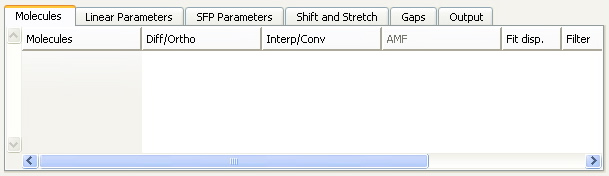
\includegraphics[width=\textwidth]{img/Quickstart_CalibrationMolecule.jpg}

In this page, we can specify absorption cross sections to include in
the fitting procedure (absorbing correcting terms).  For best results
(and given the usually limited information content within individual
sub-windows), it is recommended to limit the number of parameters.  In
our example, we do not include cross sections in the fit.  In the UV
region, it is sometimes necessary to add Ring and ozone.  In this
case, proceed as follows.  First try and fit the cross section term(s)
freely, looking at the retrieved values in each interval.  The usual
situation is that spectral signatures are such that the information
content largely differs from one interval to another.  Look at results
in the `best windows', and fix the absorber amount to a mean value
derived from these particular intervals.  Although this way of working
implicitly assumes that the molecule absorption is constant over the
whole calibration interval (which is not necessarily true), this is
usually the best compromise.

\begin{minipage}{\textwidth}
\subsubsection{Linear Parameters}
\hfill\vspace{-.8\baselineskip}
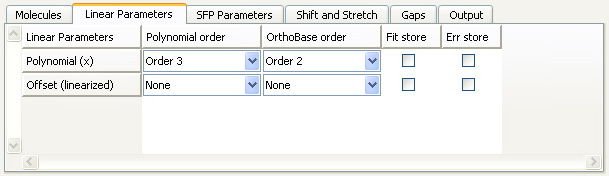
\includegraphics[width=\textwidth]{img/Quickstart_CalibrationLinear.jpg}
\end{minipage}\\

The smooth component of the differential absorbance is fitted by a polynomial.  The degree of the polynomial may be adjusted according
to the size of sub-windows and the quality of the fit.  The orthogonal base is used to calculate differential cross sections (not present
in this example).

\begin{minipage}{\textwidth}
\subsubsection{SFP Parameters}
\hfill\vspace{-.8\baselineskip}
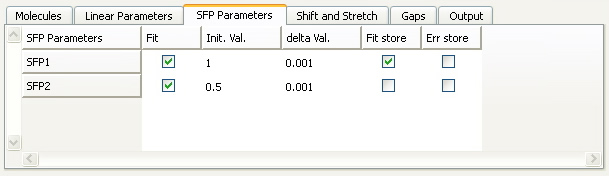
\includegraphics[width=\textwidth]{img/Quickstart_CalibrationSFP.jpg}
\end{minipage}
\glspl{sfp} are defined in this page.

In the example, the selected line shape is a gaussian.  The parameter
to fit is the \gls{fwhm} which is represented by SFP1.  The other
parameter SFP 2 is ignored for this type of line shape even though it
is checked.

Again in this case, a better accuracy is obtained when limiting the number of free parameters according to the information
content of spectra.  For line shapes involving two parameters such as the error function, which is the convolution between
a Gaussian (SFP 1) and a boxcar (SFP 2), it is recommended to fix the value of one (or several) parameters in order to optimize
the algorithm.  Several iterations may be needed.

\begin{minipage}{\textwidth}
\subsubsection{Shift and Stretch}
\hfill\vspace{-.8\baselineskip}
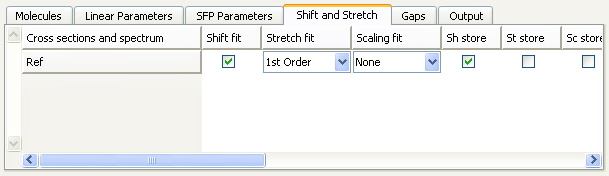
\includegraphics[width=\textwidth]{img/Quickstart_CalibrationShift.jpg}
\end{minipage}

Shift (and stretch) can be applied either on the control spectrum
(symbol \textbf{Spectrum} in this case) or on the solar spectrum
(symbol \textbf{Ref} in this case).  In order to avoid interpolating
the control spectrum, we recommend to shift the high-resolution solar
spectrum instead of the control one (see equation \ref{eq:gaussian},
section \ref{sec:wavel-calibr}).  \emph{Note that, in this case, the
  cross section(-s) defined in the \textbf{Molecules} page must be
  shifted together with the solar spectrum.}

Right-click the \textbf{Insert} or \textbf{Modify} option to add a new item in the list or to modify a selection.

\subsection{Analysis Window Properties}
To create a `new Analysis Windows' item in the \textbf{Projects} tree, select the predefined
\textbf{`Analysis Windows'} node (or an existing analysis window to add the new one after) and right-click
the \textbf{``New Analysis Windows..."} command.  Give it a name and right-click the properties option from the new
analysis windows item to have the following dialog box.

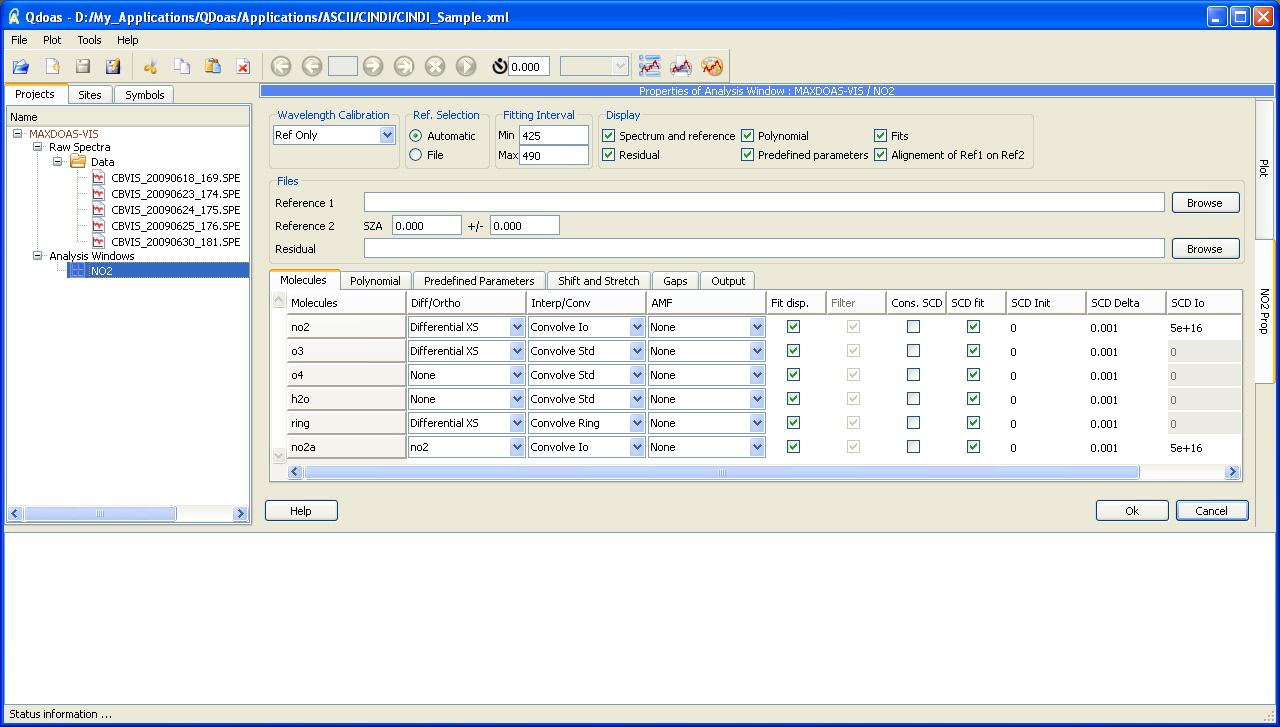
\includegraphics[width=\textwidth]{img/Quickstart_Analysis.jpg}

\subsubsection{Analysis Windows Properties}

The recommended \textbf{fitting interval} for \NO2 in the visible region is 425-490 nm.

We have checked the option \textbf{Automatic} in the \textbf{Reference selection} frame.  This means that a reference spectrum is automatically selected every day from the current data file.  If both values are not zero, the spectrum will be different for each twilight.  In the example, the spectrum measured at the minimum solar zenith angle of the day is selected.

The wavelength calibration is applied on the reference spectrum (here, \textbf{Reference 2}).  If a file had also been specified in \textbf{Reference 1}, it would have had  the priority for the wavelength calibration and the shift between both \textbf{Reference 1} and \textbf{Reference 2} would have been determined in order align cross sections on \textbf{Reference 2} before the analysis of spectra.

The structure of the \textbf{Analysis Windows Properties} pages is very similar to the one used for the calibration (and already defined above).

\subsubsection{Molecules}
\hfill\vspace{-.8\baselineskip}
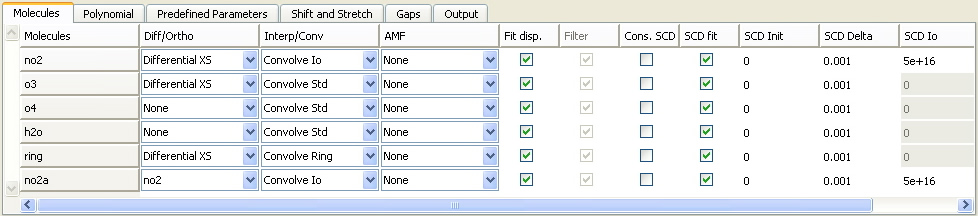
\includegraphics[width=\textwidth]{img/Quickstart_AnalysisMolecules.jpg}

This page contains the absorption cross sections needed for \NO2 retrieval (see the list, page \pageref{sec:no2_settings}).  Differential cross sections
are generated by orthogonalisation to an orthogonal base defined in the \textbf{Polynomial} page.  In order to avoid correlation between cross sections
(e.g. NO2 and NO2a) of similar shapes (e.g. when treating temperature effects by including two or several cross sections of the same species),
these cross sections can be orthogonalised with respect to each other.  High-resolution cross sections are convolved using the information
on the calibration and the slit function retrieved from the wavelength calibration procedure.  \NO2 cross sections are convolved using $I_0$ correction
(see page \pageref{sec:no2_settings}); a typical concentration of $5e16$ is used.

\subsubsection{Polynomial}
\hfill\vspace{-.8\baselineskip}
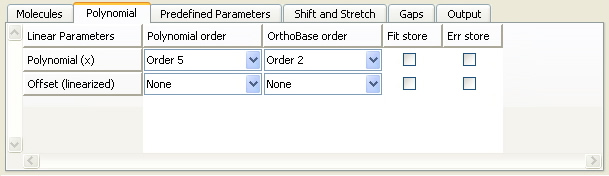
\includegraphics[width=\textwidth]{img/Quickstart_AnalysisLinear.jpg}

In this page, the polynomial used for fitting the smooth part of the absorbance is defined.  An orthogonal base is built with the main components of the polynomial in order to calculate differential cross sections.

\subsubsection{Predefined Parameters}
\hfill\vspace{-.8\baselineskip}
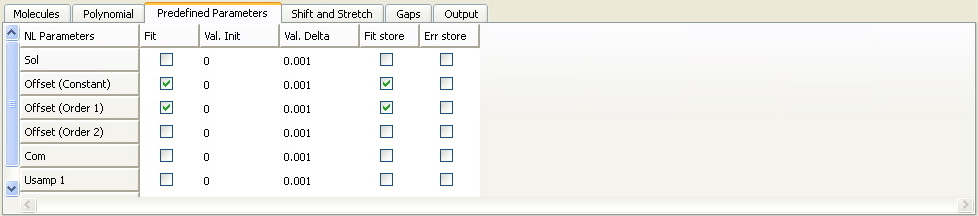
\includegraphics[width=\textwidth]{img/Quickstart_AnalysisPredefined.jpg}

Predefined parameters page contains reserved symbols not defined by the user (for example, offset).

\subsubsection{Shift and Stretch}
\hfill\vspace{-.8\baselineskip}
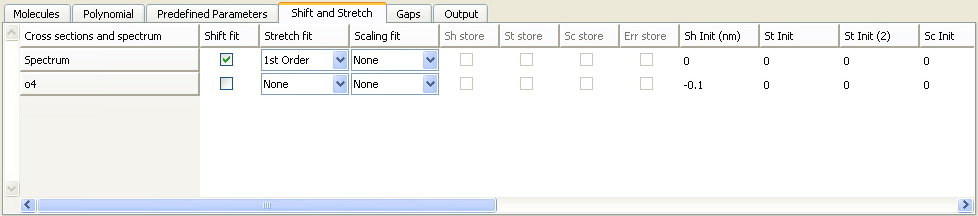
\includegraphics[width=\textwidth]{img/Quickstart_AnalysisShift.jpg}

Shift and stretch (1st order) applied to the spectrum are fitted here.  In this page, a shift value is also applied (not fitted) to the \tetraox~cross section.  Note that several cross sections can be grouped together.  Right-click the \textbf{Insert} or \textbf{Modify} option to add a new item or to modify the selection.

\subsection{Running Analysis}

To analyse a spectra file, select it in the \textbf{Projects} tree and right-click the \textbf{Run Analysis} command.

\begin{tabular}{p{1.5cm} p{10cm}}
\textbf{Note}	& if you right-click \textbf{Run Analysis} command from a parent node (\textbf{Data} folder or \textbf{Raw Spectra}), the command will be applied on all spectra files defined in the selected project.
\end{tabular}

The analysis of a record is processed in one shot (even if several analysis windows are defined) and the results of the fit are plotted in different pages.  The panel at the bottom of the user interface provides information related to the type of plot currently displayed.

\begin{minipage}{\textwidth}
\subsubsection{Kurucz page}
\hfill\vspace{-.8\baselineskip}
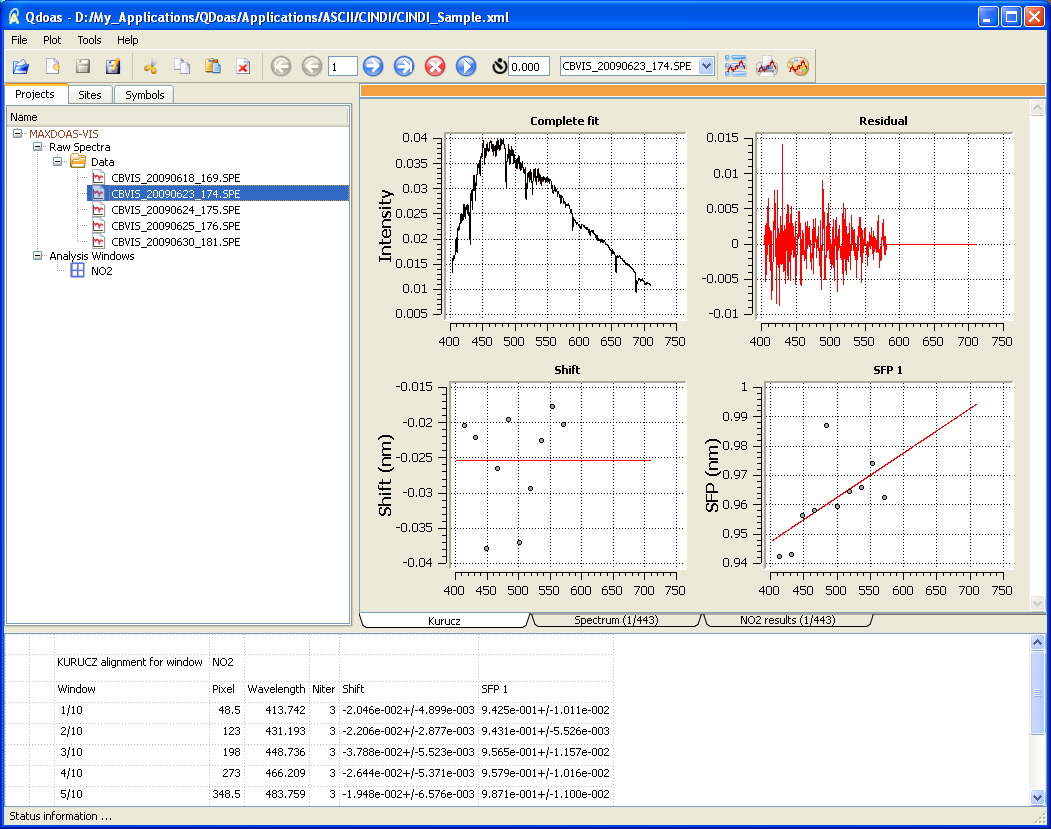
\includegraphics[width=\textwidth]{img/Quickstart_RunAnalysis.jpg}
\end{minipage}\\

This page appears in front of the others when the first spectrum is processed.  It contains the plots resulting from the wavelength calibration procedure~:

\begin{qdoasitem}
\item \textbf{Complete fit}~: the selected reference spectrum (in red) is compared to the high-resolution solar spectrum convolved with the calculated resolution of the instrument (in black); if you zoom in the plot, you can check if structures match.  The wavelength calibration is the new calculated one.  It can be saved by right-clicking on the \textbf{Save As} option in order to be associated to another reference spectrum.
\item \textbf{Residual}~: the normalised residual;
\item \textbf{Shift}~: the calibration error;
\item \textbf{SFP 1}~: the variation of the \gls{fwhm} of the Gaussian with the wavelength.
\end{qdoasitem}

The red line represents the polynomial that fits individual points calculated in each sub-windows (black dots).  The whole detector wavelength range is covered.  All this information can be saved in a file using the \textbf{Save As} option.  A file with four columns is created (new wavelength calibration, polynomial fitting the individual points, wavelength at the centre of each sub-window and the calculated value for this sub-window.  Columns 3 and 4 are completed with "0" values in order to have the number of points of the detector.

\subsubsection{Spectrum page}

The currently analyzed spectrum is displayed in this page.  The panel at the bottom of the user interface provides information on the record according to the selection made in the \textbf{Selection page} of \textbf{Projects Properties}.

\subsubsection{NO2 page}
\hfill\vspace{-.8\baselineskip}
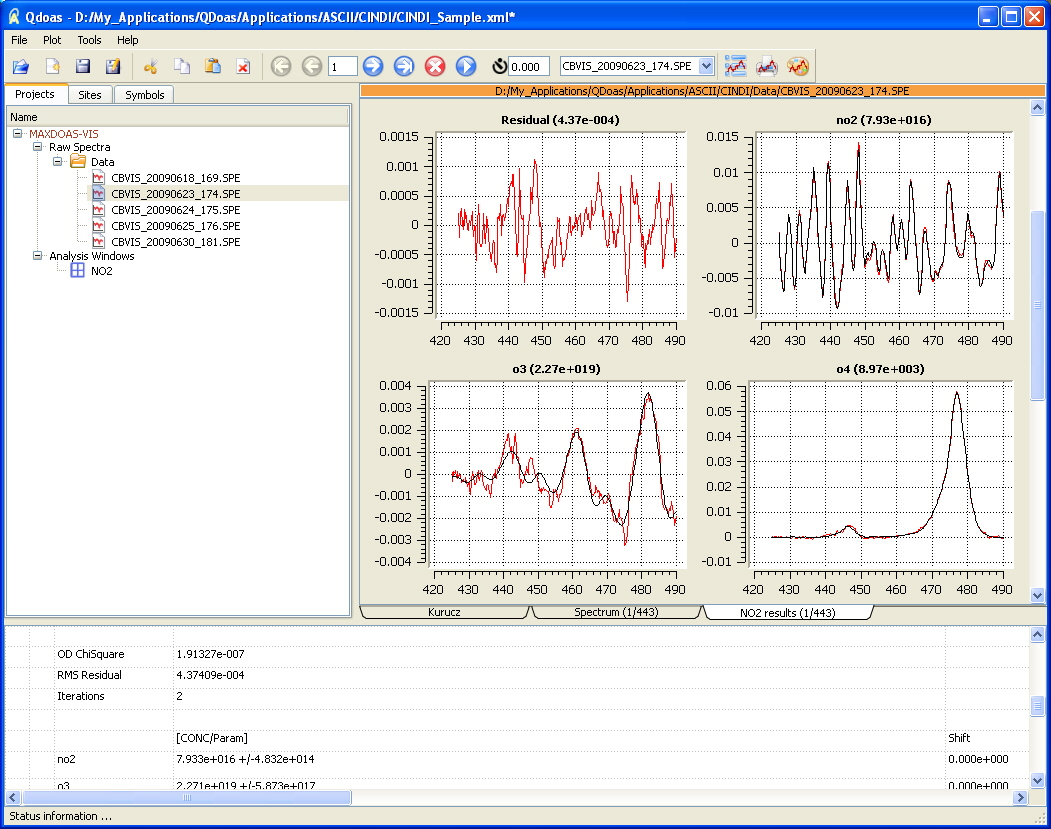
\includegraphics[width=\textwidth]{img/Quickstart_RunAnalysis_Fit.jpg}

The information on the calibration and the resolution of the instrument retrieved from the wavelength calibration procedure are used to convolve cross sections on the correct grid.   The cross sections respectively measured (the optical thickness after removal of the contribution of all molecules excepted one) and calculated (the remaining cross section multiplied by the calculated slant column density) are displayed.

\subsubsection{Output}
% add screenshot?
To save the results, stop the current analysis using the red button in the toolbar, open \textbf{Projects Properties}, and go to the \textbf{Output} page.  In order to save results, check ``Analysis'' and choose the location and format of the output file(-s).  Check ``Calibration'' to save reference spectrum calibration results as well.  Still on the \textbf{Output} page, you may select various other fields to be saved to the output file.  Next, go to the \textbf{Analysis Window Properties} to select molecule densities and other analysis results that should be saved to output.  To select which calibration data should be saved, go to the \textbf{Calibration} page of the \textbf{Projects Properties} window.

%%% Local Variables:
%%% mode: latex
%%% TeX-master: "QDOAS_manual"
%%% TeX-PDF-mode: t
%%% End:
